\documentclass{xtupaper}
\usepackage[urlcolor=blue]{hyperref}
\usepackage{threeparttable}
\usepackage{setspace}
\usepackage{titlesec}
\usepackage{float}
\newcommand{\upcite}[1]{\textsuperscript{\textsuperscript{\cite{#1}}}}
\usepackage{fancyhdr}
\titleformat{\section}{\large \heiti}{\chinese{section}、}{0em}{}
\begin{document}
\begin{center}
\LARGE
  \textbf{线性方程组求解——最速下降法}\\
  \vspace{0.5em}
  \large
湘潭大学,\ 数学与计算科学学院,\ 21级王艺博
  \end{center}
\rule[0.1\baselineskip]{\textwidth}{0.5pt}

\section{思路转变}
A为对称正定矩阵,$$Ax=b$$

求解向量$x$这个问题可以转化为一个求$f(x)$极小值点的问题, 为什么可以这样
$$f(x) = \frac{1}{2}x^TAx-x^Tb+c$$

可以发现 $$\nabla f=\mathrm{grad}f=Ax-b$$

由 $A$的正定性可以保证 $f(x)$的驻点一定是极小值点.而$Ax-b=0$ 得到的就是$f(x)$的驻点.
即
$$f(x^{*})=\min f(x)\quad\Leftrightarrow\quad\nabla f(x^{*})=Ax^{*}-b=0$$

把解线性方程组的问题,转化为求函数$f(x)$的极小值点.
\section{最速下降法}
\paragraph{怎么找到这个极小值点?}
已知一个多元函数沿其负梯度方向函数值下降得最快.

\noindent 一种较为形象的解释:

想象自己在半山腰上,要到山脚处:
\begin{itemize}
  \item 首先要找好下降方向:负梯度方向
  \item 之后沿着选定方向直走
  \item 走到不能再下降为止(也就是选定方向的最低点),停下来, 再找新的下降方向
  \item 重复上面的过程,便能到达山脚
\end{itemize}

\paragraph{翻译成数学语言}

\begin{itemize}
\item 给定任意初值 $x_0$,计算残量 $r_0=b-Ax_0$.
\item 选择 $P=r_0$ 为前进方向,计算
$$\alpha=\frac{\left(r_0,r_0\right)}{\left(Ar_0,r_0\right)},\quad x_1 = x_0 + \alpha r_0$$ 
\item 重复上面的过程.
\end{itemize}

算法如下:

\begin{algorithm}[ht]
  \caption{最速下降法解线性方程组}
  \label{alg:Framwork}
  \begin{algorithmic}
\State 输入:系数矩阵 $A$, 右端向量 $b$, 初值 $x0$, 容许误差 e\_tol, 最大迭代步 $N$;

\State 输出:数值解 $x$

  \State $k=0$;
\State 计算残量 $r=b-Ax0$;
\While {$\|r\|>$e\_tol \& $k<N$}
    \State $\alpha=\frac{\left(r,r\right)}{\left(Ar,r\right)}$;
    \State $x = x0 + \alpha * r$;
    \State $x0 = x$;
    \State $r=b-Ax0$;
    \State $k=k+1$;
\EndWhile        
   \If {$k>N$}
      \State 输出: 算法超出最大迭代次数;
   \Else
      \State 输出: 迭代次数 $k$;
   \EndIf
   \State 返回 $x$;
  \end{algorithmic}
\end{algorithm}


\section{北太天元源程序}
\paragraph{最速下降法解线性方程组}
\lstinputlisting[language=matlab]{../Gradient_Descent.m}
将上述代码保存为 \verb|Gradient_Descent.m| 文件。

\section{数值算例}
下面例子中统一 $ N=100,e\_tol=10^{-8},x_0 = 0  $ 

\begin{example}
  $$Ax=b$$
  $$
  A=\begin{bmatrix}
  4 & 1 & 0 & 0 \\
  1 & 4 & 1 & 0 \\
  0 & 1 & 4 & 1 \\
  0 & 0 & 1 & 4
  \end{bmatrix}\quad b= \begin{bmatrix}
    6 \\
    25 \\
    -11 \\
    15
    \end{bmatrix}
  $$
  用最速下降法求$ x $ ;
\end{example} 
\paragraph{实现}
\begin{lstlisting}[language=matlab]
  clc;clear all,format long;
  N = 100; e_tol = 1e-8;
  A = [  4,  1,  0,  0; 
         1,  4,  1,  0;  
         0,  1,  4,  1; 
         0,  0,  1,  4;  ]
  b=[6; 25; -11; 15];
  x0=[0; 0; 0; 0];
  [x11,k1,r11] = Gradient_Descent(A,b,x0,e_tol,N)
  x_exact = gsem_column(A,b)
  % 作图查看误差变化
  n = length(b);
  k1 = k1+1;
  % 数值解
      figure(1);
      plot(1:k1,x11(1,:),'-*r',1:k1,x11(2,:),'-og', 1:k1,x11(3,:),'-+b',1:k1,x11(4,:),'-dk');
      legend('x_1','x_2','x_3','x_4');
      title('每个数值解的变化')
  % 残差变化
      figure(2);
      plot(1:k1,r11,'-*r');
      legend('残差');
      title('残差变化')
\end{lstlisting}
运行后得到
\begin{figure}[ht]
  \centering
  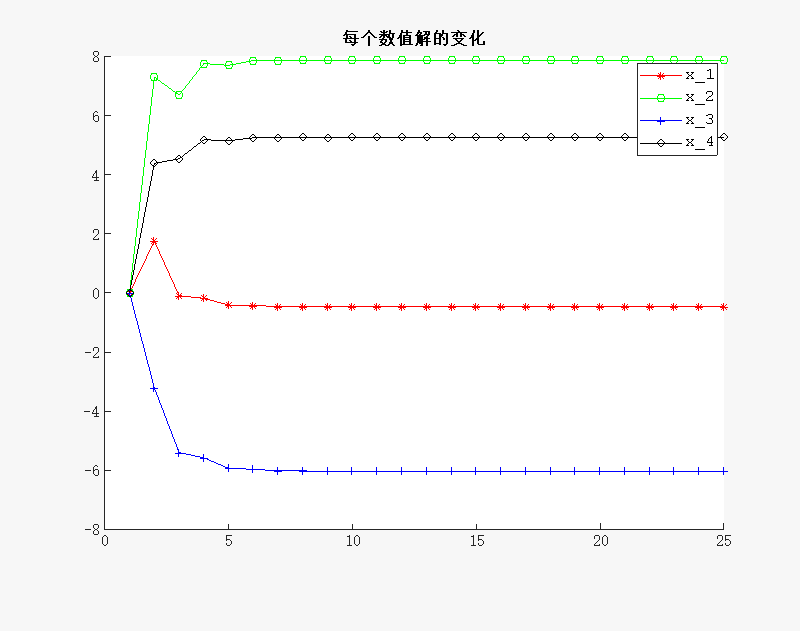
\includegraphics[scale=0.5]{../figures/fig1.png}
  \caption{}
\end{figure}

\begin{figure}[ht]
  \centering
  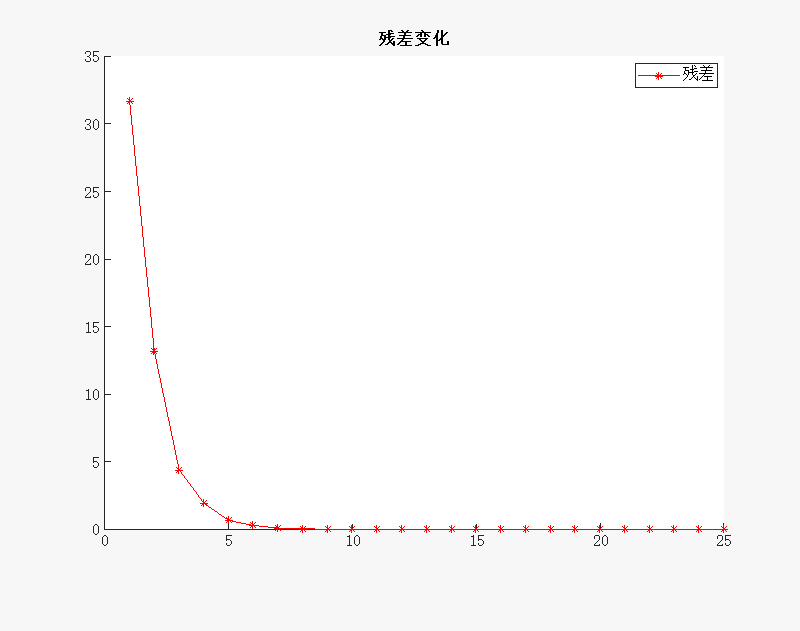
\includegraphics[scale=0.5]{../figures/fig2.png}
  \caption{}
\end{figure}
通过这个例子可以初步看到方法是可行的. 

\newpage
下面这个例子我将形象展示最速下降法的实现特点
\begin{example}
  A = [3  1; 1 5]; 
b = [-1;1];
c = 0; 
对应函数:$$f(x,y)=\frac{1}{2}\left(3x^2+2\cdot1\cdot xy+5y^2\right)-(-x+y)+0$$
\end{example}

\paragraph{三维表示一下}
\begin{lstlisting}[language=matlab]
clc;clear all;format long;
A = [3  1; 1 5]; 
b = [-1;1];
c = 0; 
N = 100; e_tol = 1e-8; x0 =zeros(length(b),1);

%x0 =[-0.1;-0.1]

x = linspace(-1,1,100); 
y = linspace(-1,1,100);
% 网格化、方便作图
[x, y] = meshgrid(x,y);
% 定义函数 f(x) = 0.5 * x' * A * x - x'*b + c
% 为了作图方便,如下定义
f=@(x,y) 0.5 * (A(1,1) * x.^2 + 2 * A(1,2) * x .* y + A(2,2) * y.^2) - (b(1) * x + b(2) * y) + c;
z = f(x,y);

mesh(x,y,z)
[x11,k1,r11] = Gradient_Descent(A,b,x0,e_tol,N);

figure(1)
mesh(x,y,z)
hold on
% 绘制最速下降法的每次迭代点
%scatter3(x11(1, :), x11(2, :), f(x11(1,:),x11(2,:)),'r','filled');
plot3(x11(1, :), x11(2, :), f(x11(1,:),x11(2,:)),'r-o');

xlabel('x');
ylabel('y');
zlabel('f(x, y)');
title('函数的三维表示');
hold off;
\end{lstlisting}
运行后得到
\begin{figure}[htpb]
  \centering
  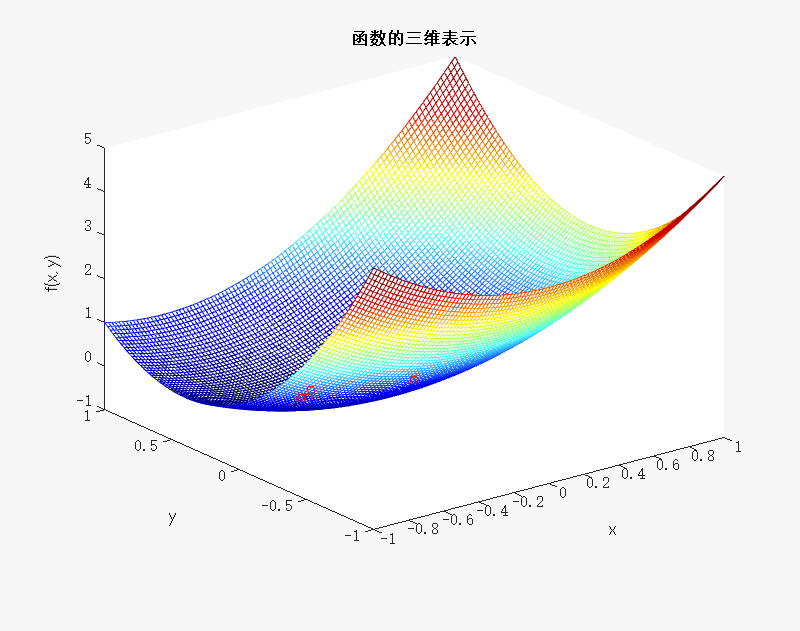
\includegraphics[scale=0.5]{../figures/fig3.png}
  \caption{}
\end{figure}

\newpage
\paragraph{绘制等高线图}
\begin{lstlisting}[language=matlab]
figure(2)
hold on 
contour(x,y,z,200)
plot(x11(1, :), x11(2, :), 'r-o');
title('最速下降法特点');
colorbar;
\end{lstlisting}
运行后得到
\begin{figure}[ht]
  \centering
  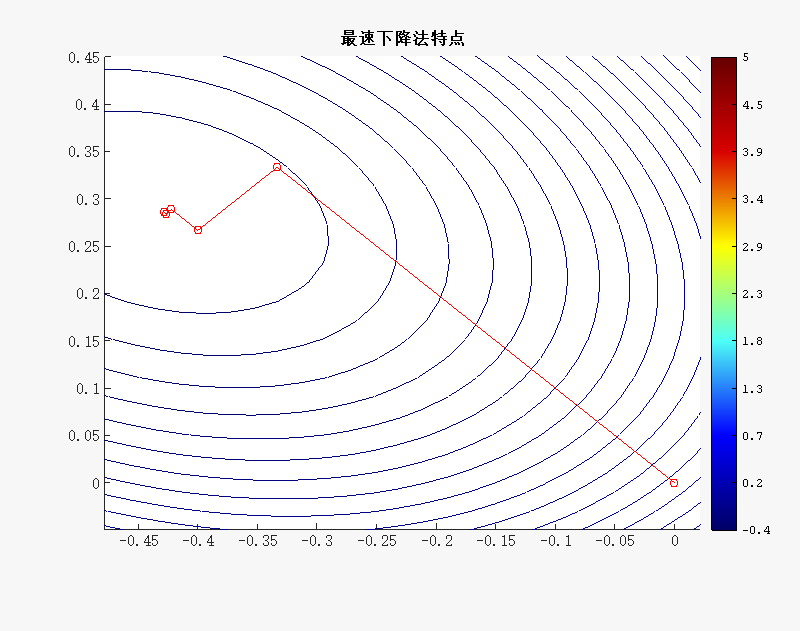
\includegraphics[scale=0.5]{../figures/fig4.png}
  \caption{}
\end{figure}

为了展示更清晰,将 $ x_0 $设为 [-0.2;0] ,可以得到这样的图像
\begin{figure}[ht]
  \centering
  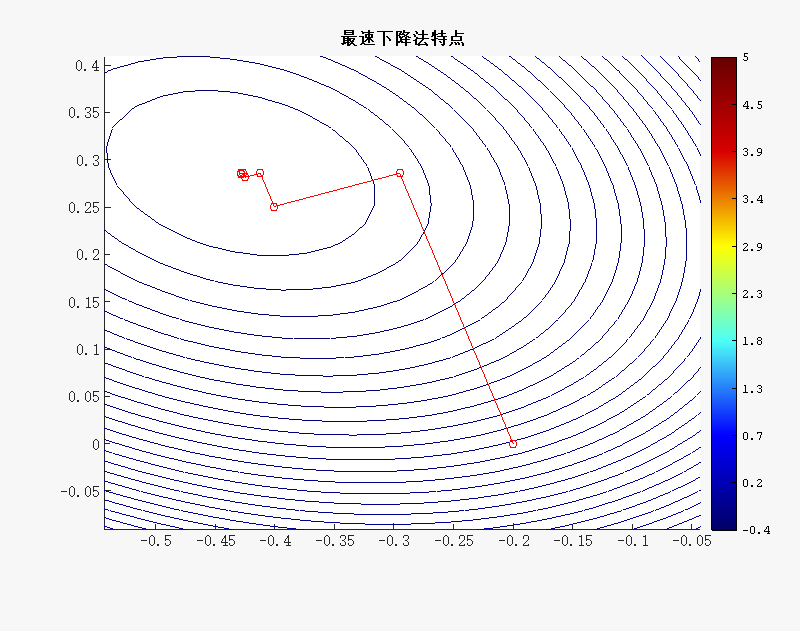
\includegraphics[scale=0.5]{../figures/fig5.png}
  \caption{}
\end{figure}


由图形可以看出,最速下降法是如何下降的.

从某一点,选定最快的下降方向,下降到不能再下降为止,再重新找新的最快的下降方向.就这样依次进行下去.

由此可以看出最速下降法的优点是容易理解和实现较为简单.当然也可以看出它还存在很大的改进空间,在每一次选方向时,明明有着更快更好的方向(三角形任意的第三边都更快).
\end{document} 

